\chapter{Συνδεσμολογία}

\subsection{Μικροελεγκτής AVR}

Σύμφωνα με τον \textcite[1]{myklebust97}, οι μικροελεγκτές AVR διαθέτουν
μειωμένο σύνολο εντολών, δηλαδή είναι υπολογιστές RISC (\te{Reduced Instruction
Set Computer}). Το χαρακτηριστικό αυτό απλοποιεί τα απαιτούμενα κυκλώματα
ελέγχου και τους παρέχουν μικρότερους κύκλους για την εκτέλεση κάθε εντολής
\parencite[1]{sequin82}. Επιπροσθέτως, οι μικροελεγκτές AVR βασίζονται σε
τροποποιημένη αρχιτεκτονική Harvard σύμφωνα με την οποία, και σε αντίθεση με την
κατά Von Neumann αρχιτεκτονική, το πρόγραμμα και τα δεδομένα τοποθετούνται σε
ανεξάρτητα φυσικά μέσα που χαρακτηρίζονται, μεταξύ άλλων, από ανεξάρτητους
διαύλους πρόσβασης \parencite[1]{myklebust97}.

Άμεσα πλεονεκτήματα αυτού του σχεδιασμού είναι ότι καθίσταται δυνατή η
ταυτόχρονη πρόσβαση στις μνήμες προγράμματος και δεδομένων στον ίδιο κύκλο
\parencite[8]{atmel13}. Επιπλέον, επιτρέπεται η χρήση διαφορετικών τεχνολογιών
για κάθε μνήμη. Για παράδειγμα, στην περίπτωση του χρησιμοποιούμενου
μικροελεγκτή, ATmega328, τα δεδομένα οργανώνονται σε μνήμη πλάτους των 8bit
τεχνολογίας SRAM (\te{Static RAM}) με 2KiB συνολική χωρητικότητα, ενώ οι
εντολές, σε μνήμη Flash των 32KiB με θέσεις των 16bit
\parencite[8--9,16,18]{atmel13}.


Η μνήμη Flash του μικροελεγκτή χωρίζεται σε δύο περιοχές λογισμικού, την περιοχή
του προγράμματος (\te{Application section}) και την περιοχή του λογισμικού
\te{Boot loader} (\te{Boot Loader Section} -- BLS) \parencite[269]{atmel13}.
Η περιοχή προγράμματος φέρει τον κώδικα που εκτελεί ο μικροελεγκτής κατά την
τυπική του λειτουργία· τον κώδικα της υλοποίησης. Στην περιοχή BLS εναποτίθεται
λογισμικό το οποίο μπορεί να εγγράψει και να διαβάσει τη μνήμη Flash με δεδομένα
που μεταφέρονται μέσω κάποιας διαθέσιμης διεπαφής του μικροελεγκτή (για
παράδειγμα, USART ή SPI), που, τυπικά, χρησιμοποιείται για την εναπόθεση του
νέου κώδικα του προγράμματος \parencite[269,273]{atmel13}.

Η εκτέλεση του \te{Boot loader} πραγματοποιείται είτε με την μεταπήδηση (εντολές
JMP ή CALL) στην περιοχή BLS από την περιοχή προγράμματος, είτε μέσω μίας
ρύθμισης του μικροελεγκτή που προκαλεί τη χρήση ως ρουτίνα εξυπηρέτησης της
διακοπής επανεκκίνησης (\te{Reset}), την πρώτη διεύθυνση της περιοχής BLS αντί
της πρώτης εντολής του προγράμματος, \parencite[273]{atmel13}. Από εκεί, το
λογισμικό \te{Boot loader} είναι υπεύθυνο να αποφασίσει εάν απαιτείται εγγραφή
νέου κώδικα στην περιοχή προγράμματος ή απευθείας μεταπήδηση πίσω σε αυτήν.


\subsection{Πλατφόρμα Arduino}
\label{subsec:arduino}

Οι πλακέτες Arduino επιλύουν τα παραπάνω ζητήματα και παρέχουν μία έτοιμη
λειτουργική μονάδα που επιτρέπει την άμεση ενασχόληση με τη δημιουργία του
πρότυπου λογισμικού και εκείνων των συνδέσεων με ηλεκτρονικά στοιχεία που
απαιτούνται στο πλαίσιο αυτού.

Για την ύπαρξη αρκετής ευελιξίας κατά το σχεδιασμό της υλοποίησης (και λόγω
έλλειψης πρότερης εμπειρίας και, επομένως, κρίσης), επιλέγεται η (πλέον
πρόσφατη, την περίοδο εκπόνησης) πλακέτα Arduino Uno revision 3, της οποίας ο
κεντρικός μικροελεγκτής είναι ένας AVR ATmega328P της Atmel. Ο συγκεκριμένος
μικροελεγκτής διαθέτει συνολική μνήμη προγράμματος 32KiB, 2KiB κύρια μνήμη,
συχνότητα ρολογιού που φτάνει τα 20MHz (που, ωστόσο, λόγω της πλακέτας,
περιορίζεται στα 16MHz) και πληθώρα δυνατοτήτων
\parencites[1]{atmel13}{arduino:uno}. Επιπροσθέτως, η πλακέτα παρέχει διασύνδεση
USB για την επικοινωνία του μικροελεγκτή με τον υπολογιστή, τόσο για τον
προγραμματισμό του όσο και για την ανταλλαγή δεδομένων με κάποια άλλη εφαρμογή,
για παράδειγμα τερματικό.

Ο μικροελεγκτής της πλακέτας \te{Arduino Uno revision 3} διατίθεται με
προεγκατεστημένο
λογισμικό \te{Boot loader} επιτρέποντας, με αυτόν τον τρόπο, τον προγραμματισμό
της μνήμης προγράμματος χωρίς τη χρήση ειδικού υλικού, αλλά με την απευθείας
σύνδεση της πλακέτα μέσω καλωδίου USB \parencite{arduino:environ}. Περισσότερα
σχετικά με το λογισμικό \te{Boot loader} αναφέρονται στην ενότητα
\nameref{subsec:avr:progmem} σ.~\pageref{subsec:avr:progmem}.
Ωστόσο, σημειώνεται ότι η
επικοινωνία μέσω USB επιτυγχάνεται με ένα δεύτερο μικροελεγκτή της πλακέτας --
ενός ATmega16U2 -- του οποίου μοναδικός σκοπός είναι η διασύνδεση του
πρωτοκόλλου USB (το οποίο υποστηρίζει εγγενώς) με το κύκλωμα USART που διαθέτει,
τόσο ο ίδιος, αλλά, κυρίως, ο ATmega328P -- ο κεντρικός μικροελεγκτής της
πλακέτας \parencites{arduino:uno}[148,185]{atmel12}[172]{atmel13}. Σαφώς, αυτή η
διασύνδεση χρησιμοποιείται για κάθε επικοινωνία μεταξύ υπολογιστή και πλακέτας
μέσω καλωδίου USB, ανεξαρτήτως εάν τα δεδομένα προορίζονται για το λογισμικό
\te{Boot loader} ή το ίδιο το πρόγραμμα.

Για την περαιτέρω διευκόλυνση της ανάπτυξης του λογισμικού του μικροελεγκτή της
πλακέτας,
παρέχεται ορισμένο επιπρόσθετο λογισμικό \te{Arduino} το οποίο λαμβάνει δύο
μορφές. Μία εξ αυτών είναι το περιβάλλον ανάπτυξης \te{Arduino IDE} του οποίου
οι βασικές λειτουργίες είναι η μεταγλώττιση του πηγαίου κώδικα και η μεταφορά
του προγράμματος στο μικροελεγκτή \parencite{arduino:environ} μέσω μίας
περισσότερο ελκυστικής γραφικής διεπαφής. Μία δεύτερη μορφή
λογισμικού είναι οι βιβλιοθήκες \te{Arduino} οι οποίες παρέχουν εύχρηστες
προγραμματιστικές διεπαφές (API) που εσωτερικά κάνουν χρήση των υποκείμενων
κυκλωμάτων του μικροελεγκτή της εκάστοτε πλακέτας (είτε απευθείας, είτε μέσω
τρίτου λογισμικού) αποκρύπτοντας, με αυτόν τον τρόπο, τις λεπτομέρειες της
υλοποίησης \parencite{arduino:lib}.


\subsection{Περιβάλλον ανάπτυξης της υλοποίησης}

Παρότι το IDE και οι βιβλιοθήκες Arduino μπορούν να επιταχύνουν σημαντικά τη
διαδικασία ανάπτυξης της υλοποίησης, προτιμάται, αντί αυτών, η απευθείας χρήση
καθιερωμένων εργαλείων για τον προγραμματισμό μικροελεγκτών AVR, καθώς έτσι
επιδιώκεται να επιτευχθεί σε μεγαλύτερο βάθος κατανόηση της συνολικής
διαδικασίας που, ιδανικά, θα επιτρέψει τη μελλοντική ενασχόληση με παρόμοια
συστήματα ανεξαρτήτως της πορείας των προϊόντων \te{Arduino}. Στο πλαίσιο της
υλοποίησης, χρησιμοποιείται μόνο το υλικό, δηλαδή η πλακέτα \te{Arduino} για την
κάλυψη των βασικών ηλεκτρικών αναγκών, και το λογισμικό \te{Boot loader} για τον
προγραμματισμό του μικροελεγκτή.

Το IDE αντικαθίσταται από έναν οποιοδήποτε επεξεργαστή κειμένου και ο πηγαίος
κώδικας διασπάται σε διαφορετικά αρχεία για την καλύτερη οργάνωσή του.
Με τον τρόπο αυτό, καθώς η υλοποίηση επεκτείνεται και ο κώδικάς της διογκώνεται,
ο λογικός διαχωρισμός των λειτουργιών της επιτρέπει το γρηγορότερο εντοπισμό
κάποιας συγκεκριμένης υπομονάδας. Επιπλέον, καθώς η μεταγλώττιση μεγάλου όγκου
πηγαίου κώδικα μπορεί να αποβεί χρονοβόρα, η ύπαρξη αυτόνομων αρχείων
αντικείμενου κώδικα δημιουργημένων από προηγούμενο κύκλο μεταγλώττισης,
επιτρέπει την επαναχρησιμοποίησή τους για την παραγωγή ενός (νέου) συνολικού
δυαδικού αρχείου, απαιτώντας μεταγλώττιση μόνο των αρχείων εκείνων που έχουν
τροποποιηθεί.


\subsubsection{Εργαλεία AVR GCC}

Η μεταγλώττιση των επιμέρους αρχείων πηγαίου κώδικα σε αντικείμενα προγράμματα
και η, εν συνεχεία, σύνδεση (ή συνένωσή) τους σε ένα τελικό δυαδικό αρχείο
αναλαμβάνεται από την AVR GNU συλλογή μεταγλωττιστών avr-gcc και λοιπών
εργαλείων της avr-binutils (όπως ο συνδέτης ld ο οποίος χρησιμοποιείται
εσωτερικά από την avr-gcc).

Το παραγόμενο δυαδικό αρχείο της σύνδεσης είναι μορφής ELF (\te{Executable and
Linking Format}) η οποία, παρότι παρέχει ανεξαρτησία από επεξεργαστή και
αρχιτεκτονική υπολογιστή, είναι, ωστόσο ακατάλληλη για την απευθείας μεταφορά
στο μικροελεγκτή AVR \parencites[47]{cruz97}[346]{avrlibc}. Απαιτείται, πρώτα, η
εξαγωγή των τμημάτων (\te{segment}) του κώδικα και των δεδομένων (\@.\te{text}
και \@.\te{data}, αντίστοιχα) από το αρχείο ELF σε ένα αρχείο δεκαεξαδικής
μορφής (αρχείο HEX) · εργασία η οποία αναλαμβάνεται από το εργαλείο avr-objcopy
\parencite[13,346]{avrlibc}.

\begin{figure}
    \caption{Η αλυσίδα εργαλείων AVR GCC για τον προγραμματισμό του
    μικροελεγκτή.\label{fig:avr:toolchain}}
    \begin{center}
    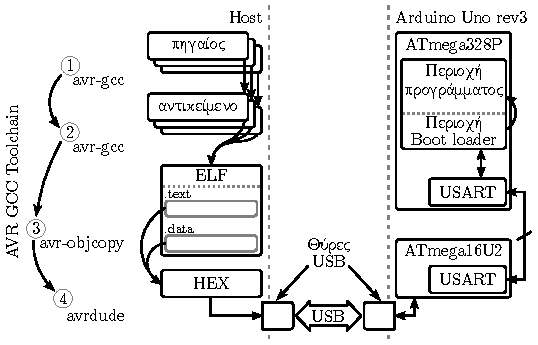
\includegraphics{avr_toolchain}
    \end{center}
\end{figure}

Τέλος, το δεκαεξαδικό αρχείο περνάει στο μικροελεγκτή μέσω του εργαλείου
avrdude, το
οποίο υποστηρίζει προγραμματισμό μικροελεγκτών AVR μέσω διαφόρων προγραμματιστών
(συμπεριλαμβανομένου ειδικών εξαρτημάτων όπως οι STK500 και AVRISP mkII της
Atmel) και, σαφώς, μέσω \te{Boot loader} \parencites[15]{avrlibc}{avrdude}.

Στο σχήμα \ref{fig:avr:toolchain} παρουσιάζεται η αλυσίδα (\te{toolchain}) των
χρησιμοποιούμενων εργαλείων που αναλαμβάνουν τα στάδια για τη μεταφορά του
πηγαίου κώδικα ως πρόγραμμα στο μικροελεγκτή. Σημειώνεται ότι το \te{Arduino
IDE} κάνει, στην πραγματικότητα, χρήση αυτών των εργαλείων με το επιπρόσθετο
χαρακτηριστικό ότι παρέχει και κάποιες άλλες διευκολύνσεις στους, αρχάριους,
χρήστες για τους οποίους προορίζεται \parencite{arduino:build}.


Κατά την εκκίνηση της συσκευής, δηλαδή κατά τη σύνδεσή της με την παροχή
τροφοδοσίας, εκτελείται η αρχικοποίηση των διαφόρων υποσυστημάτων της υλοποίησης
και, εν συνεχεία, ο μικροελεγκτής μεταπίπτει σε κατάσταση χαμηλής κατανάλωσης
ισχύος. Από αυτήν, ενεργοποιείται αυτόματα είτε για την εκκίνηση ενός νέου
κύκλου μετρήσεων (βλ. \nameref{sec:task} σ.~\pageref{sec:task}), είτε για την
εξυπηρέτηση κάποιου εισερχόμενου αιτήματος HTTP (βλ. \nameref{%
sec:network:impl-resources} σ.~\pageref{sec:network:impl-resources}). Στο σχήμα
\ref{fig:mcu:tasks} παρουσιάζεται ο κύκλος καθηκόντων του μικροελεγκτή.

\begin{figure}
    \caption{Καθήκοντα του μικροελεγκτή.\label{fig:mcu:tasks}}
    \begin{center}
    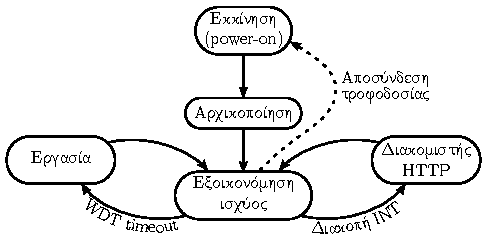
\includegraphics{mcu_tasks}
    \end{center}
\end{figure}

Αναλυτικότερα, κατά το στάδιο της αρχικοποίησης, τίθεται η συχνότητα του
ρολογιού του μικροελεκτή, η οποία, για τις ανάγκες της υλοποίησης, μειώνεται από
τα 16MHz στα 4MHz και η κατεύθυνση των ακροδεκτών (δηλαδή ποιοι είναι εισόδου
και ποιοι εξόδου). Επίσης, ρυθμίζεται το κύκλωμα WDT (\te{Watch-Dog Timer}), το
οποίο είναι υπεύθυνο για την περιοδική αφύπνιση του μικροελεγκτή ώστε να
ελέγχεται η ανάγκη εκκίνησης νέου κύκλου μετρήσεων.

Επιπλέον, ανακτώνται οι μεταβλητές ρυθμίσεις της συσκευής είτε από τις
προκαθορισμένες (εργοστασιακές ρυθμίσεις), είτε από τις αποθηκευμένες τιμές της
εφεδρικής μνήμης, εφόσον αυτές είναι έγκυρες (βλ \nameref{subsec:backup-memory}
σ.~\pageref{subsec:backup-memory}).
Οι ρυθμίσεις αυτές περιλαμβάνουν τη δικτύωση της συσκευής (διεύθυνση IP, μάσκα
υποδικτύου, προεπιλεγμένη πύλη), το λειτουργικό εύρος του υποσυστήματος κίνησης
(βλ. \nameref{sec:motor:coordinates} σ.~\pageref{sec:motor:coordinates}), το
χρονικό διάστημα μεταξύ κύκλων εργασίας καθώς και το πλήθος μετρήσεων που
πραγματοποιείται σε κάθε κύκλο (βλ. \nameref{sec:task} σ.~\pageref{sec:task}).
Ο τρόπος ρύθμισης της συσκευής περιγράφεται στους Πόρους υλοποίησης (σ.~%
\pageref{sec:network:impl-resources}).

Στην πορεία, οι ρυθμίσεις προωθούνται στις κατάλληλες μονάδες και εκτελούνται
επιπρόσθετες προετοιμασίες, όπως η παλιννόστηση της κεφαλής, δηλαδή η επαναφορά
της στη θέση επιστροφής (συντεταγμένες [0, 0, Z\tsub{max}]) (βλ. σ.~%
\pageref{sec:motor:homing}) και η αρχικοποίηση του HTTP \te{Socket} (βλ. σ.~%
\pageref{ssubsec:network:port_mr}).


\subsection{Κατάσταση χαμηλής κατανάλωσης}

Ο μικροελεγκτής διαθέτει διαφορετικές καταστάσεις νάρκης (\te{sleep mode}
όπου η καθεμία απενεργοποιεί ορισμένα κυκλώματα για τη μείωση της κατανάλωσης.
Για παράδειγμα, η πιο απλή, είναι η κατάσταση αδράνειας (\te{idle}) κατά την
οποία απενεργοποιείται μόνο το ρολόι της CPU και της μνήμης Flash (δηλαδή, της
μνήμης προγράμματος). Στο πλαίσιο της υλοποίησης, γίνεται προσπάθεια για την
ύψιστη μείωση της κατανάλωσης κατά τα διαστήματα όπου ο μικροελεγκτής παραμένει
άεργος.

Για το σκοπό αυτό, εφαρμόζεται η κατάσταση \te{power-down} κατά την οποία
απενεργοποιούνται όλα τα ρολόγια του μικροελεγκτή (clk\tsub{CPU}, clk%
\tsub{FLASH}, clk\tsub{IO}, clk\tsub{ADC}, clk\tsub{ASY}) καθώς και οι
ταλαντωτές του συστήματος και των Χρονομετρητών\slash{}Απαριθμητών \parencite%
[38]{atmel13}. Σύμφωνα με την \textcite[38]{atmel13}, ο μικροελεγκτής είναι
δυνατό να επανέλθει σε κανονική λειτουργία μόνο μέσω των ακροδεκτών INT1:0 με
παρατεταμένο λογικό 0 (\te{low-level interrupt}) καθώς και μέσω των κυκλωμάτων
TWI (\te{Two-Wire Interface}) και WDT (\te{Watch-Dog Timer}).

Στο πλαίσιο της υλοποίησης χρησιμοποιείται ο πρώτος και ο τελευταίος τρόπος· το
κύκλωμα TWI αφυπνίζει το μικροελεγκτή όταν αυτός ρυθμίζεται με ρόλο \te{slave}
στο δίαυλο TWI και κάποιο εξωτερικό κύκλωμα προσπαθεί να επικοινωνήσει μαζί του
ενώ, στην υλοποίηση, χρησιμοποιείται μόνο ως \te{master} για την επικοινωνία με
το ρολόι πραγματικού χρόνου (RTC) (βλ. \nameref{sec:rtc} σ.~\pageref{sec:rtc}).

Για την ακρίβεια, ο ένας εκ των δύο ακροδεκτών INT1:0 συνδέεται με τον ακροδέκτη
\nbar{INT} του ολοκληρωμένου δικτύωσης, W5100, το οποίο τον θέτει και τον
διατηρεί σε λογικό 0 έως ότου διευθετηθούν όλες οι ενδείξεις διακοπών που του
έχουν ενεργοποιηθεί
(βλ. \nameref{subsec:network:interface} σ.~\pageref{subsec:network:interface}).
Για τις ανάγκες της υλοποίησης, αυτό σημαίνει ότι έχει καταφθάσει εισερχόμενο
αίτημα HTTP το οποίο διεκπεραιώνεται από το διακομιστή (βλ.
\nameref{sec:http-server} σ.~\pageref{sec:http-server}).

Ο χρονομετρητής WDT ρυθμίζεται ώστε να αφυπνίζει το μικροελεγκτή κάθε 8s (το
μέγιστο διάστημα που υποστηρίζεται από τον παρόντα μικροελεγκτή) και αποτελεί το
έναυσμα για την εκκίνηση νέου κύκλου εργασιών
(\nameref{ssubsec:task:initiate} σ.~\pageref{ssubsec:task:initiate}).







